\chapter{Loop Elements}

The same basic loop circuit, shown in figure \ref{fig:loop_schematic}, is duplicated 64 times to create the full array.
Here, I will discuss the purpose and function of each part of this circuit.

\section{Active Detuning}
The loop is a resonant circuit that is strongly coupled to the volume surrounding it. It is necessary to spoil this
resonance during the high power RF transmit pulses so that excessive currents are not induced in the loop. Such
unintended energy deposition could adversely affect transmit homogenaity, damage the array, or create a safety hazard.
This selective detuning is acheived by switching an inductor across one of the loop capacitors, creating a parallel
resonant tank that behaves as an open circuit in the loop at $\omega_L$.

A DC bias current of about $120mA$ is injected on the line marked BIAS in figure \ref{fig:loop_schematic}. This bias
current flows through a PIN diode, $D_1$, creating an RF short and effectively switching $L_{TRAP}$ across $C_{S3}$.
$L_{TRAP}$ is an adjustable air core inductor, and is hand tuned to resonate with $C_{S3}$ at precisely $\omega_L$. The 
parallel resonant circuit thus formed creates a virtual open ciruit in the loop, preventing current from flowing. As 
soon as the bias current is removed and the diode recovers, the trap is disabled and the loop once again becomes tuned.

\section{Passive Detuning}
The active detuning strategy is sufficient for assurance of image quality and protection from hardware damage, but a
passive method is required to ensure patient safety in the event of an electrical failure. The crossed diode pair $D_2$
clamps the voltage across $C_{S3}$ and $L_{TRAP}$ to safe levels, passively enabling the trap if the energy stored in
the loop gets too high. Other designs might also include RF fuses in the loop circuit, but the loops employed in this
array are all small enough that this was not necesarry.

\begin{figure}
    \centering
    \input{figures/loop_diagram.pdf_tex}
    \caption{Complete loop circuit schematic}
    \label{fig:loop_schematic}
\end{figure}

\section{Loop Model}
The essence of the wire loop receive elements used in this array is a damped series resonant circuit, shown in figure
\ref{fig:loop_model} A. The loop has a distributed inductance by nature of its geometry, and is broken at regular
intervals by discrete capacitors.  Wire and component resistances and (more importantly) inductive coupling to adjacent
conductive materials reduces the loop Q to a finite value. This effect is modelled by a series resistor with value
$R_{LOAD}=\sqrt{\frac{L}{C}}\cdot\frac{1}{Q}$

\section{Complete Loop Circuit}
Figure \ref{fig:loop_model} B shows the creation of an output port in the loop circuit. The total loop capacitance is split into $C_P$, 
across which the output port is formed, and $C_S$. A series capacitor $C_M$ is added to one terminal of the output port.
For the purpose of further analisys, it is convenient to lump component impedances together into three blocks: $Z_P$ (parallel
imedance), $Z_S$ (series impedance), and $Z_M$ (matching impedance). These impedances are defined in figure \ref{fig:loop_model} C.

\begin{figure}
    \centering
    \input{figures/loop_model.pdf_tex}
    \caption{Loop circuit models}
    \label{fig:loop_model}
\end{figure}

\section{Loop Circuit Analisys}
The loop ciruit has an input inpedance of $Z_{IN}$ at its port, as defined in equation \ref{eq:Z_IN}. This impedance can
be split into its real and imaginary parts, $R_{IN}$ and $X_{IN}$, shown in equations \ref{eq:R_IN} and \ref{eq:X_IN}.

\begin{equation} \label{eq:Z_IN}
    Z_{IN}=(jX_p)\parallel(jX_S+R_{LOAD})+jX_M = \frac{j X_P (j X_S + R_L)}{j (X_P + X_S) + R_L} + j X_M
\end{equation}

\begin{equation} \label{eq:R_IN}
    R_{IN}=Re(Z_{IN})=\frac{{X_P}^2 R_L}{{R_L}^2+(X_P+X_S)^2}
\end{equation}

\begin{equation} \label{eq:X_IN}
    X_{IN}= Im(Z_{IN}) = \frac{X_P ({R_L}^2 + X_S(X_P+X_S))}{{R_L}^2+(X_P+X_S)^2}+X_M
\end{equation}

\section{Loop Component selection}

\subsection{Loop Circuit Considerations}
\subsubsection{Minimizing Preamp Noise Figure}
The vendor supplied preamplifier is designed to achieve minimum noise figure when presented with a purely real 50 ohm 
load at its input. Therefore, component values should be selected such that $R_{IN}=50\Omega$ and $X_{IN}=0\Omega$.
\subsubsection{Preamp Decoupling}
Preamp decoupling is typicall achieved by resonating a capacitor in the loop ($C_P$ in figure \ref{fig:loop_model}) with
an inductor in series with one terminal of the output port (in the same position as $C_M$ in figure
\ref{fig:loop_model}) through the input of the preamplifier. In our case, the inductance is integrated into the
preamplifier itself. I measure the inductance of the preamplifer input to be roughly $130nH$ at $123.25 MHz$. The
details of the preamp topology are unavailible to me. I simply consider it to have an impedance of $Z_{PREAMP}$, which
is transformed to ${Z_{PREAMP}}'$ (as shown in equation \ref{eq:Z_PREAMP}) by the short length of coaxial cable
connecting the preamp to the loop.

\begin{equation} \label{eq:Z_PREAMP}
    {Z_{PREAMP}}'=Z_0 \cdot \frac{Z_{PREAMP}-j Z_0 \cdot \tan(2\pi\cdot\frac{L_{COAX}}{\lambda})}{Z_0 - j Z_{PREAMP} \cdot
    \tan(2\pi\cdot\frac{L_{COAX}}{\lambda})}
\end{equation}
\begin{equation} \label{eq:X_PREAMP}
    {X_{PREAMP}}'=Im({Z_{PREAMP}}')
\end{equation}
    
In any case, preamp decoupling is achieved when $X_P+X_M+{X_{PREAMP}}'=0$

\subsection{Loop Resonance}
I define loop resonance as occuring at a frequency $\omega_0$ where $X_P + X_S = 0$. In this case, the equations for $R_{IN}$ and $X_{IN}$ simplify to
equations \ref{eq:R_IN_RES} and \ref{eq:X_IN_RES} respectively. It can easily be seen how $X_P$ could be selected to set
$R_{IN}$ to $50\Omega$ at resonance, but it then becomes impossible to set $X_{IN}$ to $0\Omega$ and also achieve preamp decoupling.

\subsection{Off resonance behavior}
It is not necessary that the loop be tuned to resonate precisely at the frequency of interest. The position of
$\omega_0$ relative to that of the Lamor frequency $\omega_L$ is another variable that we can manipulate to achieve the
desired loop circuit characteristics.

Consid


\begin{equation} \label{eq:R_IN_RES}
    R_{IN}\big|_{\omega_0}=\frac{{X_P}^2}{R_L} = \frac{{X_S}^2}{R_L} 
\end{equation}

\begin{equation} \label{eq:X_IN_RES}
    X_{IN}\big|_{\omega_0}=X_P+X_M=-X_S+X_M
\end{equation}

\begin{figure}
    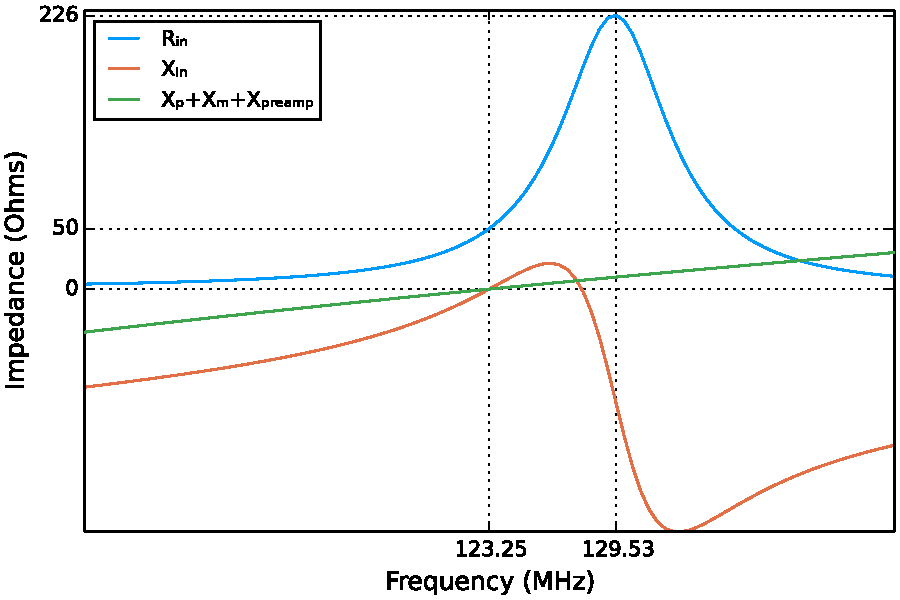
\includegraphics[width=6in]{figures/impedance_plot.pdf}
    \caption{Loop impedances vs. frequency with optimal component values}
    \label{fig:impedance_plot}
\end{figure}
